% !TEX TS-program = xelatex
% !TeX spellcheck = ru_RU
% !TEX root = talk.tex

\documentclass
  [ russian
  , aspectratio=1610
  ] {beamer}

% !TeX spellcheck = ru_RU
% !TEX root = talk.tex
% Опциональные добавления используемых пакетов. Вполне может быть, что они вам не понадобятся, но в шаблоне приведены примеры их использования.
\usepackage{tikz} % Мощный пакет для создание рисунков, однако может очень сильно замедлять компиляцию
\usetikzlibrary{decorations.pathreplacing,calc,shapes,positioning,tikzmark}

% Библиотека для TikZ, которая генерирует отдельные файлы для каждого рисунка
% Позволяет ускорить компиляцию, однако имеет свои ограничения
% Например, ломает пример выделения кода в листинге из шаблона
% \usetikzlibrary{external}
% \tikzexternalize[prefix=figures/]

\newcounter{tmkcount}

\tikzset{
    use tikzmark/.style={
            remember picture,
            overlay,
            execute at end picture={
                    \stepcounter{tmkcount}
                },
        },
    tikzmark suffix={-\thetmkcount}
}

\usepackage{booktabs} % Пакет для верстки "более книжных" таблиц, вполне годится для оформления результатов
% В шаблоне есть команда \multirowcell, которой нужен этот пакет.
\usepackage{multirow}
\usepackage{siunitx} % для таблиц с единицами измерений

% Для названий стоит использовать \textsc{}
\newcommand{\OCaml}{\textsc{OCaml}}
\newcommand{\miniKanren}{\textsc{miniKanren}}
\newcommand{\BibTeX}{\textsc{BibTeX}}
\newcommand{\vsharp}{\textsc{V$\sharp$}}
\newcommand{\fsharp}{\textsc{F$\sharp$}}
\newcommand{\csharp}{\textsc{C\#}}
\newcommand{\GitHub}{\textsc{GitHub}}
\newcommand{\SMT}{\textsc{SMT}}

\definecolor{eclipseGreen}{RGB}{63,127,95}
% \lstdefinelanguage{ocaml}{
% keywords={@type, function, fun, let, in, match, with, when, class, type,
% nonrec, object, method, of, rec, repeat, until, while, not, do, done, as, val, inherit, and,
% new, module, sig, deriving, datatype, struct, if, then, else, open, private, virtual, include, success, failure,
% lazy, assert, true, false, end},
% sensitive=true,
% commentstyle=\small\itshape\ttfamily,
% keywordstyle=\ttfamily\bfseries, %\underbar,
% identifierstyle=\ttfamily,
% basewidth={0.5em,0.5em},
% columns=fixed,
% fontadjust=true,
% literate={->}{{$\to$}}3 {===}{{$\equiv$}}1 {=/=}{{$\not\equiv$}}1 {|>}{{$\triangleright$}}3 {\\/}{{$\vee$}}2 {/\\}{{$\wedge$}}2 {>=}{{$\ge$}}1 {<=}{{$\le$}} 1,
% morecomment=[s]{(*}{*)}
% }

\makeatletter
\@ifclassloaded{beamer}{
    %%% Обязательные пакеты
    %% Beamer
    \usepackage{beamerthemesplit}
    \usetheme{SPbGU}
    \beamertemplatenavigationsymbolsempty

    %% Локализация
    \usepackage{fontspec}
    \setmainfont{CMU Serif}
    \setsansfont{CMU Sans Serif}
    \setmonofont{CMU Typewriter Text}
    %\setmonofont{Fira Code}[Contextuals=Alternate,Scale=0.9]
    %\setmonofont{Inconsolata}
    \usepackage{polyglossia}
    \setmainlanguage{russian}
    \setotherlanguage{english}

    %% Графика
    \usepackage{pdfpages} % Позволяет вставлять многостраничные pdf документы в текст

    % Математические окружения с русским названием
    \newtheorem{rutheorem}{Теорема}
    \newtheorem{ruproof}{Доказательство}
    \newtheorem{rudefinition}{Определение}
    \newtheorem{rulemma}{Лемма}
    \usepackage{fancyvrb}
}
{}
\makeatother

\usepackage[autostyle]{csquotes} % Правильные кавычки в зависимости от языка
\usepackage{totcount}
\usepackage{setspace}
\usepackage{amsmath, amsfonts, amssymb, amsthm, mathtools} % "Адекватная" работа с математикой в LaTeX

% Подпись под рисунком
\newcommand{\figcap}[1]{\par\vspace{-2pt}{\scriptsize\itshape #1\par}\vspace{4pt}}


\makeatletter

%!TEX root = talk.tex

%% Параметры заполнения титульного листа
\usepackage{xkeyval}

%% Русскоязычный вариант
\define@key[ru]{mytitle}{chair}{\def\my@title@chair@ru{#1}}
\define@key[ru]{mytitle}{title}{\def\my@title@title@ru{#1}}
\define@key[ru]{mytitle}{group}{\def\my@title@group@ru{#1}}
\define@key[ru]{mytitle}{author}{\def\my@title@author@ru{#1}}
\define@key[ru]{mytitle}{supervisor}{\def\my@title@supervisor@ru{#1}}
\define@key[ru]{mytitle}{supervisorPosition}{\def\my@title@supervisorPosition@ru{#1}}
\define@key[ru]{mytitle}{reviewer}{\def\my@title@reviewer@ru{#1}}
\define@key[ru]{mytitle}{reviewerPosition}{\def\my@title@reviewerPosition@ru{#1}}
\define@key[ru]{mytitle}{consultant}{\def\my@title@consultant@ru{#1}}
\define@key[ru]{mytitle}{consultantPosition}{\def\my@title@consultantPosition@ru{#1}}
\define@key[ru]{mytitle}{year}{\def\my@title@year@ru{#1}}
\define@key[ru]{mytitle}{specialty}{\def\my@title@specialty@ru{#1}}
\define@key[ru]{mytitle}{programme}{\def\my@title@programme@ru{#1}}
\define@key[ru]{mytitle}{profile}{\def\my@title@profile@ru{#1}}
\define@choicekey*[ru]{mytitle}{type}{coursework,practice,prediploma,master,bachelor,production}{\def\my@title@type@ru{#1}}
\define@choicekey*[ru]{mytitle}{kind}{solution,experiment,production,comparison,theoretical}{\def\my@title@kind@ru{#1}}

%% Англоязычный вариант
\define@key[en]{mytitle}{chair}{\def\my@title@chair@en{#1}}
\define@key[en]{mytitle}{title}{\def\my@title@title@en{#1}}
\define@key[en]{mytitle}{group}{\def\my@title@group@en{#1}}
\define@key[en]{mytitle}{author}{\def\my@title@author@en{#1}}
\define@key[en]{mytitle}{supervisor}{\def\my@title@supervisor@en{#1}}
\define@key[en]{mytitle}{supervisorPosition}{\def\my@title@supervisorPosition@en{#1}}
\define@key[en]{mytitle}{reviewer}{\def\my@title@reviewer@en{#1}}
\define@key[en]{mytitle}{reviewerPosition}{\def\my@title@reviewerPosition@en{#1}}
\define@key[en]{mytitle}{consultant}{\def\my@title@consultant@en{#1}}
\define@key[en]{mytitle}{consultantPosition}{\def\my@title@consultantPosition@en{#1}}
\define@key[en]{mytitle}{year}{\def\my@title@year@en{#1}}
\define@key[en]{mytitle}{specialty}{\def\my@title@specialty@en{#1}}
\define@key[en]{mytitle}{programme}{\def\my@title@programme@en{#1}}
\define@key[en]{mytitle}{profile}{\def\my@title@profile@en{#1}}
\define@choicekey*[en]{mytitle}{type}{coursework,practice,prediploma,master,bachelor}{\def\my@title@type@en{#1}}
\define@choicekey*[en]{mytitle}{kind}{solution,experiment,production,comparison,theoretical}{\def\my@title@kind@en{#1}}

\newcommand{\filltitle}[2]{
    %% Значения по умолчанию для обоих языков
    \ifthenelse{\equal{#1}{ru}}
    {
        \presetkeys[#1]{mytitle}{
            year = {\the\year},
            type = {practice},
            reviewer = {},
            consultant = {},
            profile = {}
        }{}
    }
    {}
    \ifthenelse{\equal{#1}{en}}
    {
        \presetkeys[#1]{mytitle}{
            year = {\the\year},
            type = {practice},
            reviewer = {},
            consultant = {},
            profile = {}
        }{}
    }
    {}
    \setkeys[#1]{mytitle}{#2}
}


% !TeX spellcheck = ru_RU
% !TEX root = talk.tex

%% Если что-то забыли, при компиляции будут ошибки Undefined control sequence \my@title@<что забыли>@ru
%% Если англоязычная титульная страница не нужна, то ее можно просто удалить.
\filltitle{ru}{
    %% Актуально только для курсовых/практик. ВКР защищаются не на кафедре а в ГЭК по направлению,
    %%   и к моменту защиты вы будете уже не в группе.
    chair              = {Кафедра системного программирования},
    group              = {23.Б11-мм},
    %
    %% Макрос filltitle ненавидит пустые строки, поэтому обязателен хотя бы символ комментария на строке
    %% Актуально всем.
    title              = {Анализ масштабируемости алгоритмов в D-Galois по количеству узлов},
    %
    %% Здесь указывается тип работы. Возможные значения:
    %%   production - производственная практика;
    %%   coursework - отчёт по курсовой работе (ОБРАТИТЕ ВНИМАНИЕ, у техпрога и ПИ нет курсовых, только практики);
    %%   practice - отчёт по учебной практике;
    %%   prediploma - отчёт по преддипломной практике;
    %%   master - ВКР магистра;
    %%   bachelor - ВКР бакалавра.
    type               = {practice},
    %
    %% Здесь указывается вид работы. От вида работы зависят критерии оценивания.
    %%   solution - «Решение». Обучающемуся поручили найти способ решения проблемы в области разработки программного обеспечения или теоретической информатики с учётом набора ограничений.
    %%   experiment - «Эксперимент». Обучающемуся поручили изучить возможности, достоинства и недостатки новой технологии, платформы, языка и т. д. на примере какой-то задачи.
    %%   production - «Производственное задание». Автору поручили реализовать потенциально полезное программное обеспечение.
    %%   comparison - «Сравнение». Обучающемуся поручили сравнить несколько существующих продуктов и/или подходов.
    %%   theoretical - «Теоретическое исследование». Автору поручили доказать какое-то утверждение, исследовать свойства алгоритма и т.п., при этом не требуя написания кода.
    kind               = {solution},
    %
    author             = {Власенко Даниил Сергеевич},
    %
    %% Актуально только для ВКР. Указывается код и название направления подготовки. Типичные примеры:
    %%   02.03.03 \enquote{Математическое обеспечение и администрирование информационных систем}
    %%   02.04.03 \enquote{Математическое обеспечение и администрирование информационных систем}
    %%   09.03.04 \enquote{Программная инженерия}
    %%   09.04.04 \enquote{Программная инженерия}
    %% Те, что с 03 в середине --- бакалавриат, с 04 --- магистратура.
    specialty          = {09.03.04 \enquote{Программная инженерия}},
    %
    %% Актуально только для ВКР. Указывается шифр и название образовательной программы. Типичные примеры:
    %%   СВ.5162.2020 \enquote{Технологии программирования}
    %%   СВ.5080.2020 \enquote{Программная инженерия}
    %%   ВМ.5665.2022 \enquote{Математическое обеспечение и администрирование информационных систем}
    %%   ВМ.5666.2022 \enquote{Программная инженерия}
    %% Шифр и название программы можно посмотреть в учебном плане, по которому вы учитесь.
    %% СВ.* --- бакалавриат, ВМ.* --- магистратура. В конце --- год поступления (не обязательно ваш, если вы были в академе/вылетали).
    % programme          = {СВ.5162.2021 \enquote{Технологии программирования}},
    %
    %% Актуально всем.
    %% Должно умещаться в одну строчку, допускается использование сокращений, но без переусердствования,
    %% короткая строка с большим количеством сокращений выглядит странно
    %supervisorPosition = {проф. кафeдры системного программирования, д.ф.-м.н.,}, % Терехов А. Н.
    %supervisorPosition = {ст. преподаватель кафедры ИАС, к.~ф.-м.~н. (если есть),}, % Смирнов К. К.
    %supervisorPosition = {доцент кафедры системного программирования, к.~ф.-м.~н.},
    %supervisor         = {Григорьев~С.~В.},
    %
    %% Актуально только для практик и курсовых. Если консультанта нет или он совпадает с научником, закомментировать или удалить вовсе.
    %consultantPosition = {должность, ООО \enquote{Место работы}, степень  (если есть),},
   %consultant         = {Консультант~К.~К.},
    %
    %% Актуально только для ВКР.
    % reviewerPosition   = {должность, ООО \enquote{Место работы}, степень (если есть),},
    %reviewer           = {Рецензент~Р.~Р.},
}

% Английский титульник нужен только для ВКР, остальные виды работ могут его смело игнорировать.
%\filltitle{en}{
%    chair              = {Advisor's chair},
%    group              = {ХХ.BХХ-mm},
%    title              = {Template for SPbU qualification works},
%    type               = {bachelor},
%    author             = {FirstName Surname},
    %
    %% Possible choices:
    %%   02.03.03 \foreignquote{english}{Software and Administration of Information Systems}
    %%   02.04.03 \foreignquote{english}{Software and Administration of Information Systems}
    %%   09.03.04 \foreignquote{english}{Software Engineering}
    %%   09.04.04 \foreignquote{english}{Software Engineering}
    %% Те, что с 03 в середине --- бакалавриат, с 04 --- магистратура.
%    specialty          = {02.03.03 \foreignquote{english}{Software and Administration of Information Systems}},
    %
    %% Possible choices:
    %%   СВ.5162.2020 \foreignquote{english}{Programming Technologies}
    %%   СВ.5080.2020 \foreignquote{english}{Software Engineering}
    %%   ВМ.5665.2022 \foreignquote{english}{Software and Administration of Information Systems}
    %%   ВМ.5666.2022 \foreignquote{english}{Software Engineering}
%    programme          = {СВ.5162.2020 \foreignquote{english}{Programming Technologies}},
    %
    %% Note that common title translations are:
    %%   кандидат наук --- C.Sc. (NOT Ph.D.)
    %%   доктор ... наук --- Sc.D.
    %%   доцент --- docent (NOT assistant/associate prof.)
    %%   профессор --- prof.
%    supervisorPosition = {Sc.D, prof.},
%    supervisor         = {S.S. Supervisor},
    %
%    consultantPosition = {position at \foreignquote{english}{Company}, degree if present},
%    consultant         = {C.C. Consultant},
    %
%    reviewerPosition   = {position at \foreignquote{english}{Company}, degree if present},
%    reviewer           = {R.R. Reviewer},
%}


\newcommand{\academicGroup}{\my@title@group@ru}
\newcommand{\advisorChair}{\my@title@chair@ru}
\title[Масштабируемость D-Galois]{\my@title@title@ru}
\author[\my@title@author@ru]{\my@title@author@ru, группа \academicGroup}
\institute[СПбГУ]{}
\date[2026]{}
\newcommand{\defenseYear}{\my@title@year@ru}

\makeatother

\begin{document}
{
\setbeamertemplate{footline}{}

\begin{frame}
    \vspace{15pt}
    \begin{center}
        \begin{tabular}{c}
            \scriptsize{Санкт-Петербургский государственный университет} \\
            \scriptsize{\advisorChair}
        \end{tabular}
        \titlepage
    \end{center}

    \btVFill

    \begin{center}
        \vspace{5pt}
        \scriptsize{Санкт-Петербург\\ \defenseYear}
    \end{center}
\end{frame}
}

\begin{frame}
    \frametitle{Постановка задачи}
    \textbf{Цель}: оценить масштабируемость распределённого Galois (D-Galois)
    по числу рангов на алгоритмах BFS, SSSP, TC и PageRank
    и объяснить, от чего она зависит
\end{frame}

\begin{frame}
    \frametitle{Как считает D-Galois}
    \begin{columns}[T]
        \begin{column}{.5\textwidth}
            \textbf{Разбиение OEC}: каждый ранг получает непрерывный блок номеров вершин
            (\emph{мастера}) со всеми их исходящими рёбрами. Блоки подбираются так, чтобы рёбер
            было поровну

            \medskip
            Конец ребра на чужом ранге~--- \emph{зеркало}, локальная копия чужой вершины

            \medskip
            \textbf{RF} (replication factor)~--- среднее число копий вершины по всем рангам
        \end{column}
        \begin{column}{.5\textwidth}
            \textbf{Раунд} в режиме BSP (\texttt{--exec=Sync}):
            \begin{enumerate}
                \item счёт: ранг проходит своих мастеров
                \item sync: зеркала отправляют изменения мастерам
                \item Allreduce: осталась ли работа у кого-нибудь
            \end{enumerate}

            \medskip
            Следующий раунд начинается, когда все ранги закончили предыдущий
        \end{column}
    \end{columns}
\end{frame}

\begin{frame}
    \frametitle{Стенд и методика}
    \begin{columns}[T]
        \begin{column}{.45\textwidth}
            \textbf{Оборудование}
            \begin{itemize}
                \item Intel Core i7-10750H: 6 ядер, 12 потоков, 8~ГБ DDR4
                \item Ubuntu 24.04, GCC 13.3, Open MPI 4.1.6
                \item Galois, коммит \texttt{b67f9420}
            \end{itemize}
        \end{column}
        \begin{column}{.55\textwidth}
            \textbf{Методика}
            \begin{itemize}
                \item $P = 1\ldots6$ MPI-рангов по 1 потоку, каждый на своём ядре
                      (\texttt{--map-by core --bind-to core})
                \item Режим \texttt{--exec=Sync}, \texttt{-t=1}
                \item Время~--- медиана прогонов внутри Galois
                      (\texttt{-runs=10} для BFS и SSSP, \texttt{-runs=15} для
                      PageRank и TC), без чтения и разбиения графа
                \item Для BFS и SSSP источник~--- вершина медианной степени
                \item Промахи кэшей~--- \texttt{perf stat}
                      (L1-dcache-load-misses, LLC-load-misses)
                \item Граф фиксирован, растёт число рангов $P$:
                      ускорение $S(P) = T(1)/T(P)$, идеал $S(P) = P$
            \end{itemize}
        \end{column}
    \end{columns}
\end{frame}

\begin{frame}
    \frametitle{Набор данных}
    \begin{center}
        \footnotesize
        \setlength{\tabcolsep}{4.5pt}
        \begin{tabular}{lrrrlr}
            \toprule
            Граф & Вершин & Рёбер & Ср. степень & Тип графа & RF ($P=6$) \\
            \midrule
            belgium\_osm      & 1\,441\,295 & 3\,099\,940  & 2.15 & дорожный  & 1.18 \\
            roadNet-CA        & 1\,971\,281 & 5\,533\,214  & 2.81 & дорожный  & 1.02 \\
            rgg\_n\_2\_22\_s0  & 4\,194\,304 & 60\,718\,396 & 14.48 & случ. геом. & 1.01 \\
            soc-LiveJournal1  & 4\,847\,571 & 68\,993\,773 & 14.23 & соцсеть   & 3.05 \\
            coPapersDBLP      & 540\,486   & 30\,491\,458 & 56.4 & соавторство & 1.82 \\
            \bottomrule
        \end{tabular}
    \end{center}

    \begin{itemize}
        \item Дорожные графы (belgium\_osm, roadNet-CA): степень вершин почти одинаковая
        \item RGG: $2^{22}$ случайных точек в квадрате, ребро~--- если точки ближе $r$
        \item LiveJournal: соцсеть, $1\%$ вершин держат существенную долю рёбер
        \item coPapersDBLP: сеть соавторства, есть хабы
    \end{itemize}
\end{frame}

\begin{frame}[shrink]
    \frametitle{Ускорение всех алгоритмов}
    \centering
    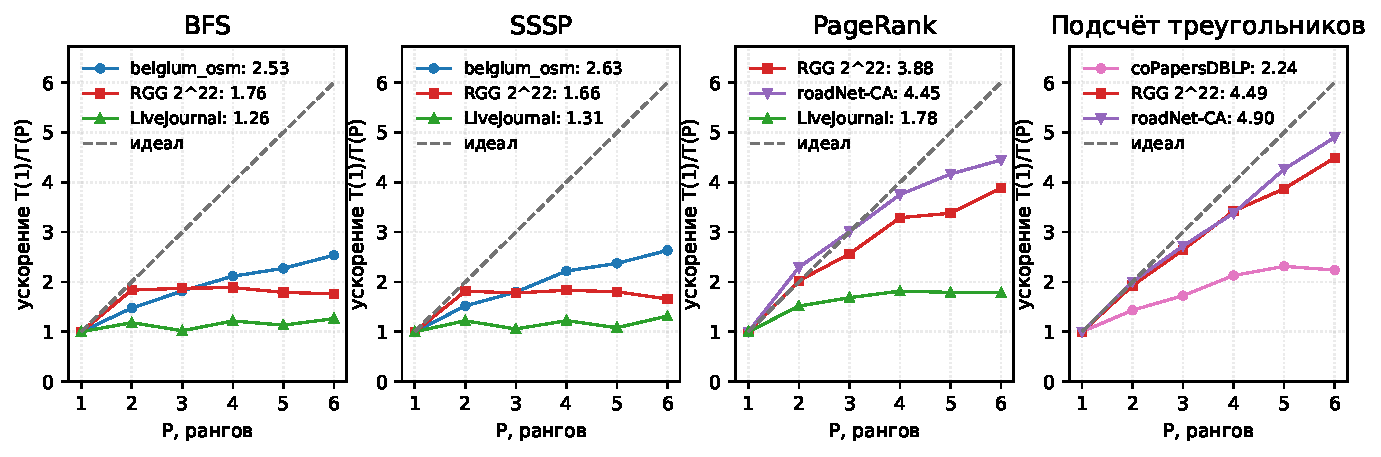
\includegraphics[width=\textwidth,height=.52\textheight,keepaspectratio]{figures/speedup_all.pdf}
    \figcap{Ускорение $S(P) = T(1)/T(P)$ при $P = 1\ldots6$ рангах, пунктир~--- идеал $S = P$,
    в легенде~--- ускорение при $P = 6$}

    \begin{itemize}
        \item Подсчёт треугольников делится почти идеально на малых графах:
              roadNet-CA $S(6) = 4.90$, RGG 4.49
        \item PageRank на roadNet-CA: $S(6) = 4.45$
        \item BFS и SSSP: $S(6) = 1.3\ldots2.6$, лучше всего на belgium\_osm
        \item Хуже всех LiveJournal: $S(6) = 1.26$ (BFS), $1.31$ (SSSP) и $1.78$ (PageRank)
    \end{itemize}
\end{frame}

\begin{frame}[shrink]
    \frametitle{BFS: время по графам}
    \centering
    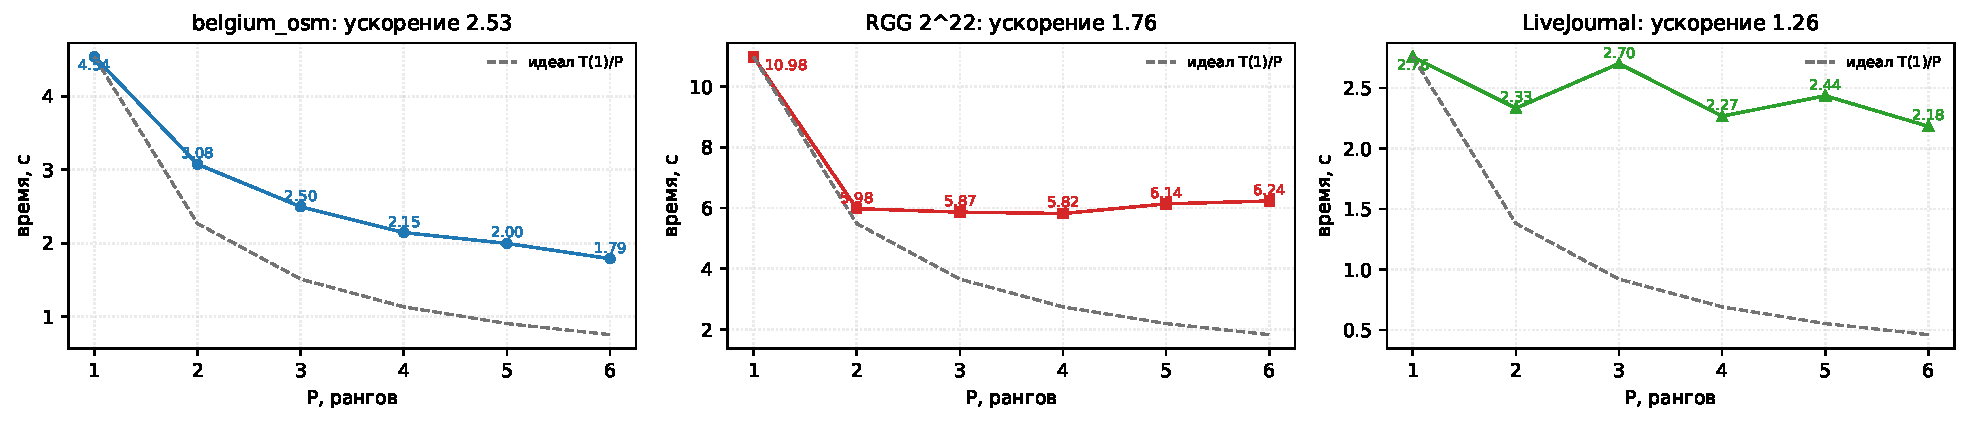
\includegraphics[width=\textwidth,height=.55\textheight,keepaspectratio]{figures/time_bfs_graphs.pdf}
    \figcap{BFS: время при $P = 1\ldots6$ рангах, своя панель на каждый граф;
    пунктир~--- идеал $T(1)/P$, в заголовке~--- ускорение при $P = 6$}

    \begin{itemize}
        \item belgium\_osm: $4.54 \to 1.79$~с, ускорение 2.53~--- лучший результат
        \item Ускорение падает с ростом средней степени: 2.5 (belgium\_osm) $\to$ 14.5 (RGG)
        \item На LiveJournal ($2.76 \to 2.18$~с) и RGG ($10.98 \to 6.24$~с) время
              перестаёт падать после $P = 2$: барьер в каждом раунде и обмен зеркалами
    \end{itemize}
\end{frame}

\begin{frame}[shrink]
    \frametitle{BFS: время по фазам при разном $P$}
    \centering
    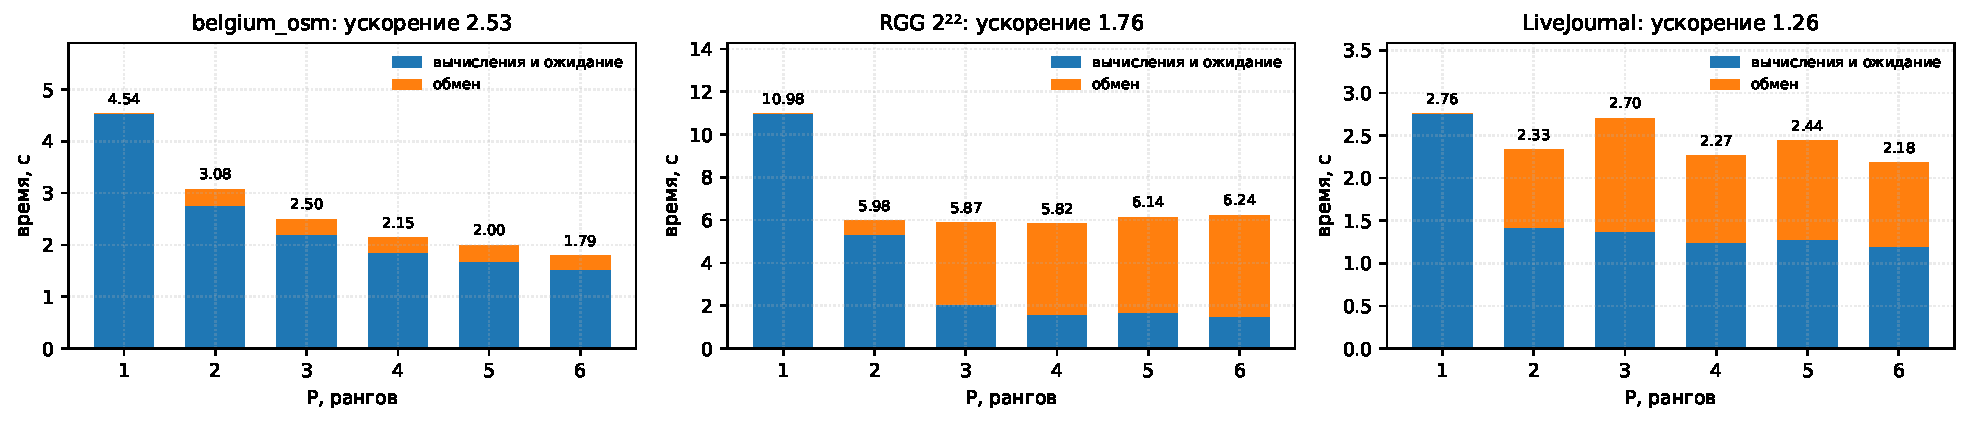
\includegraphics[width=\textwidth,height=.55\textheight,keepaspectratio]{figures/phases_bfs.pdf}
    \figcap{BFS: фазы при $P = 1\ldots6$ рангах, медиана 10 прогонов; обмен~---
    \texttt{Gluon Sync\_BFS\_*}, вычисления и ожидание~--- остаток \texttt{Timer\_N};
    над столбцом~--- время ранга (таймеры Galois пишут целые мс,
    при $P = 1$ обмен не виден)}

    \begin{itemize}
        \item belgium\_osm: обмен 10--16\%, $S(6) = 2.53$~--- деление работы перевешивает барьер
        \item RGG: уже при $P \ge 3$ обмен занимает 65--76\%, ускорение падает до 1.76
        \item LiveJournal: 39--49\% на всех $P$, $S(6) = 1.26$~--- зеркала хабов на всех рангах
    \end{itemize}
\end{frame}

\begin{frame}[shrink]
    \frametitle{BFS: промахи кэшей при разном $P$}
    \centering
    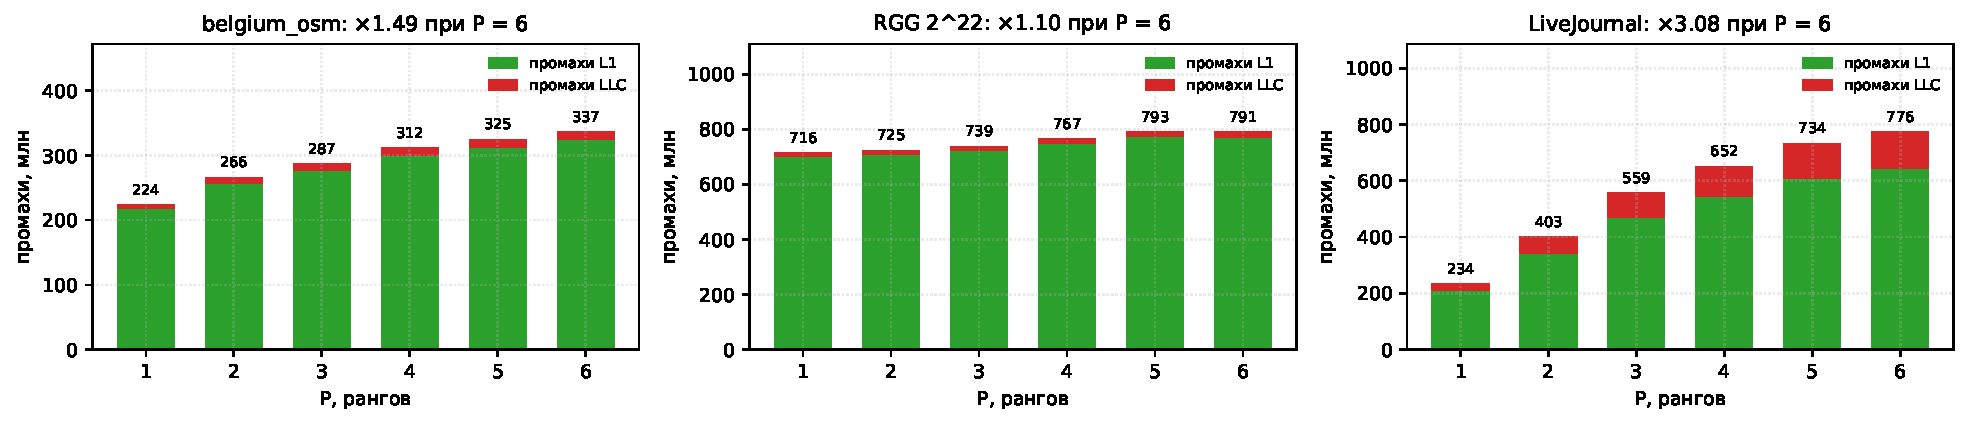
\includegraphics[width=\textwidth,height=.55\textheight,keepaspectratio]{figures/cache_bfs.pdf}
    \figcap{BFS: промахи кэшей при $P = 1\ldots6$; столбец разбит на промахи L1
    (\texttt{L1-dcache-load-misses}) и промахи LLC (\texttt{LLC-load-misses}),
    слева~--- миллионы промахов; счётчики \texttt{perf stat} снимались отдельно
    для каждого ранга, в столбце~--- их сумма; в заголовке~--- во сколько раз
    выросли промахи L1 при $P = 6$}

    \begin{itemize}
        \item belgium\_osm: промахи L1 растут с 217 до 324~млн ($\times 1.49$),
              LLC~--- с 6.1 до 13.3~млн ($\times 2.18$)
        \item RGG: промахи почти не растут ($\times 1.10$ по L1, $\times 1.24$ по LLC)
        \item LiveJournal: промахи растут втрое ($\times 3.08$) и в пять раз
              ($\times 5.24$)~--- хабы копируются на все ранги
    \end{itemize}
\end{frame}

\begin{frame}[shrink]
    \frametitle{BFS: работа по рангам при $P = 6$}
    \centering
    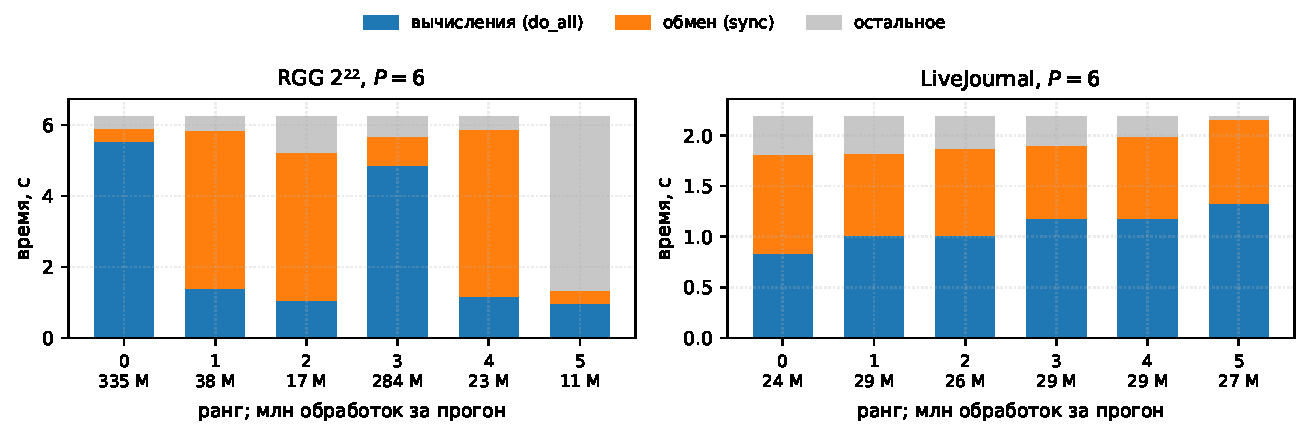
\includegraphics[width=\textwidth,height=.55\textheight,keepaspectratio]{figures/bfs_hosts.pdf}
    \figcap{BFS при $P = 6$: время фаз каждого ранга за прогон}

    \begin{itemize}
        \item RGG: ранги 0 и 3 получают 335 и 284 млн обработок, остальные~--- 11--38 млн;
              ранги 1, 2 и 4 по 4.2--4.7~с (67--76\% времени) проводят в обмене, $S(6) = 1.76$
        \item LiveJournal: обмен 0.73--0.98~с на всех рангах (33--45\% времени);
              темп задаёт ранг 5 (1.33~с вычислений)
    \end{itemize}
\end{frame}

\begin{frame}[shrink]
    \frametitle{SSSP: время по графам}
    \centering
    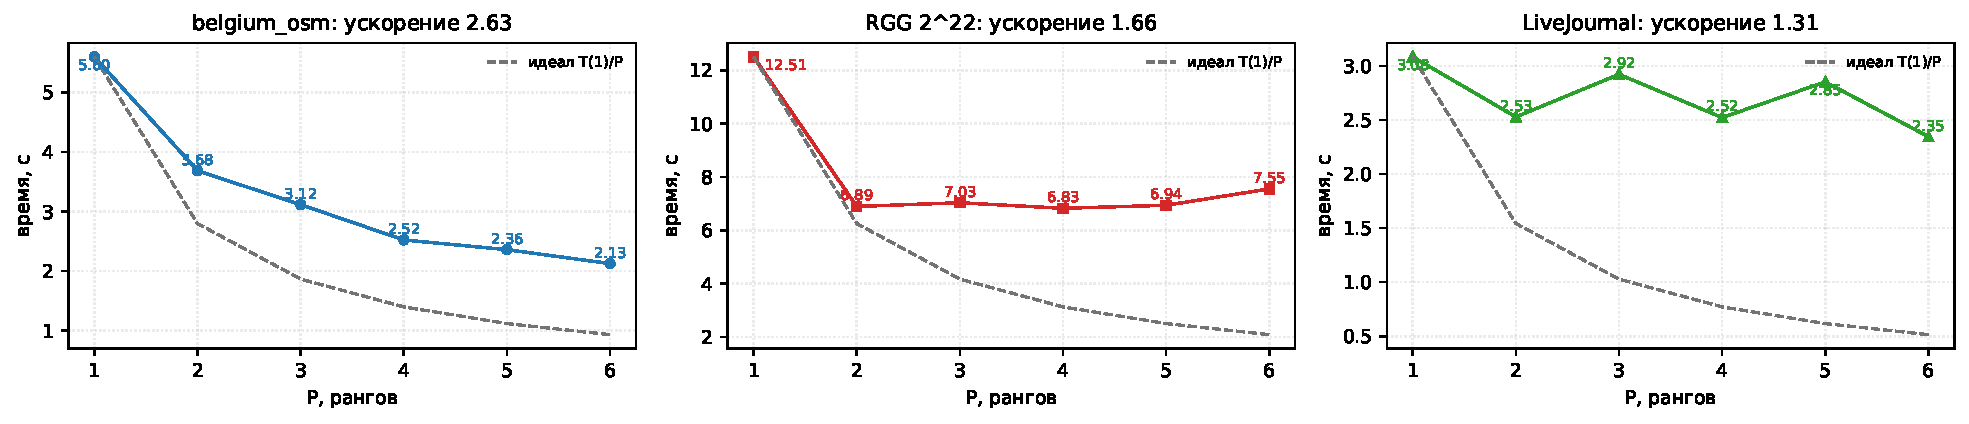
\includegraphics[width=\textwidth,height=.55\textheight,keepaspectratio]{figures/time_sssp_graphs.pdf}
    \figcap{SSSP: время при $P = 1\ldots6$ рангах, своя панель на каждый граф;
    пунктир~--- идеал $T(1)/P$}

    \begin{itemize}
        \item belgium\_osm: $5.60 \to 2.13$~с, ускорение 2.63~--- картина повторяет BFS
        \item RGG: $12.51 \to 7.55$~с, ускорение 1.66
        \item LiveJournal: $3.08 \to 2.35$~с, ускорение 1.31~--- почти не масштабируется
    \end{itemize}
\end{frame}

\begin{frame}[shrink]
    \frametitle{SSSP: время по фазам при разном $P$}
    \centering
    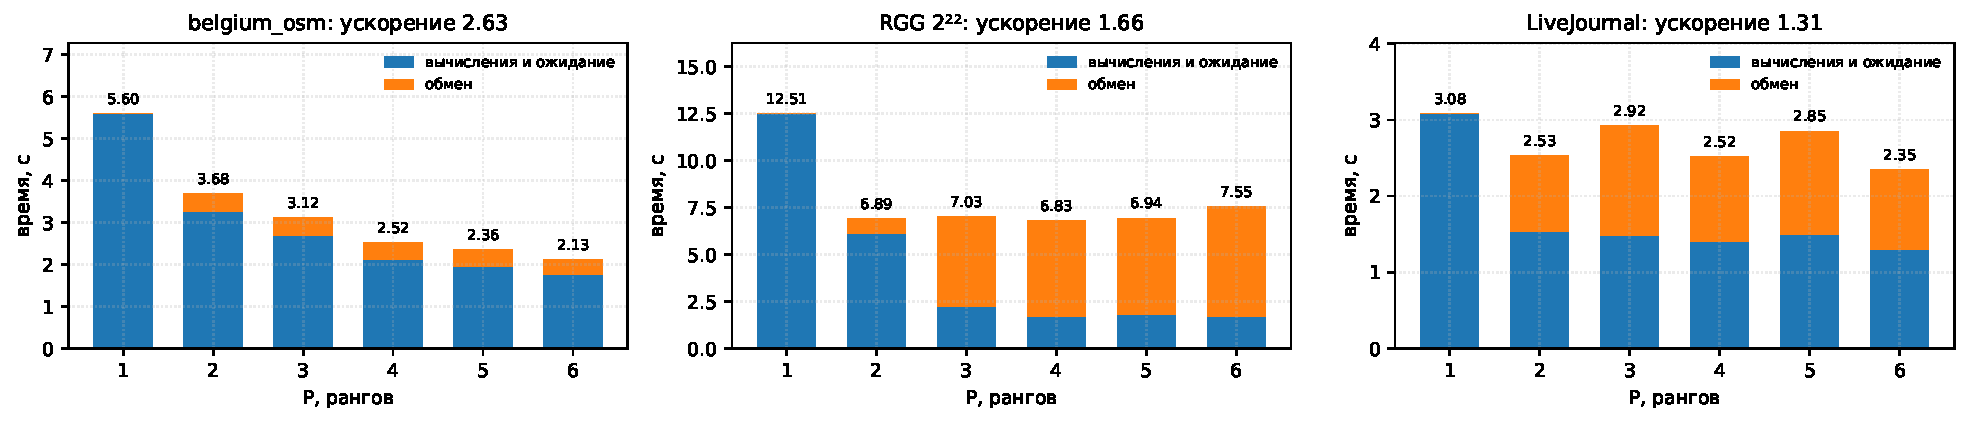
\includegraphics[width=\textwidth,height=.55\textheight,keepaspectratio]{figures/phases_sssp.pdf}
    \figcap{SSSP: фазы при $P = 1\ldots6$ рангах, медиана 10 прогонов; обмен~---
    \texttt{Gluon Sync\_SSSP\_*}, вычисления и ожидание~--- остаток \texttt{Timer\_N};
    над столбцом~--- время ранга}

    \begin{itemize}
        \item belgium\_osm: обмен 12--18\%, $S(6) = 2.63$~--- картина повторяет BFS
        \item RGG: при $P \ge 3$ обмен 68--77\%, $S(6) = 1.66$~--- как и в BFS, барьер после $P = 2$
        \item LiveJournal: 39--49\%, $S(6) = 1.31$~--- почти не масштабируется
    \end{itemize}
\end{frame}

\begin{frame}[shrink]
    \frametitle{SSSP: промахи кэшей при разном $P$}
    \centering
    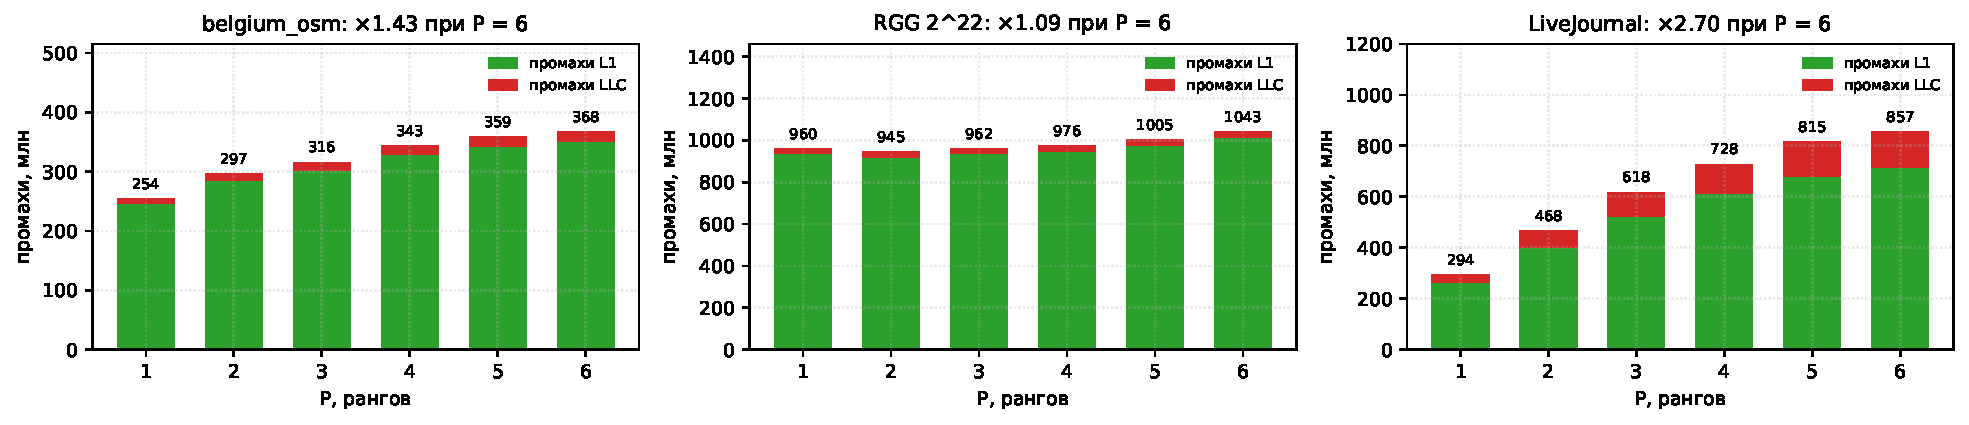
\includegraphics[width=\textwidth,height=.55\textheight,keepaspectratio]{figures/cache_sssp.pdf}
    \figcap{SSSP: промахи кэшей при $P = 1\ldots6$; столбец разбит на промахи L1
    (\texttt{L1-dcache-load-misses}) и промахи LLC (\texttt{LLC-load-misses}),
    слева~--- миллионы промахов; счётчики \texttt{perf stat} снимались отдельно
    для каждого ранга, в столбце~--- их сумма; в заголовке~--- во сколько раз
    выросли промахи L1 при $P = 6$}

    \begin{itemize}
        \item belgium\_osm: промахи L1 растут с 246 до 351~млн ($\times 1.43$),
              LLC~--- с 8.5 до 16.6~млн ($\times 1.97$)
        \item RGG: промахи почти не растут ($\times 1.09$ по L1, $\times 1.13$ по LLC)
        \item LiveJournal: промахи растут в 2.7 раза ($\times 2.70$) и почти
              в пять раз ($\times 4.77$)~--- картина повторяет BFS
    \end{itemize}
\end{frame}

\begin{frame}[shrink]
    \frametitle{PageRank: время по графам}
    \centering
    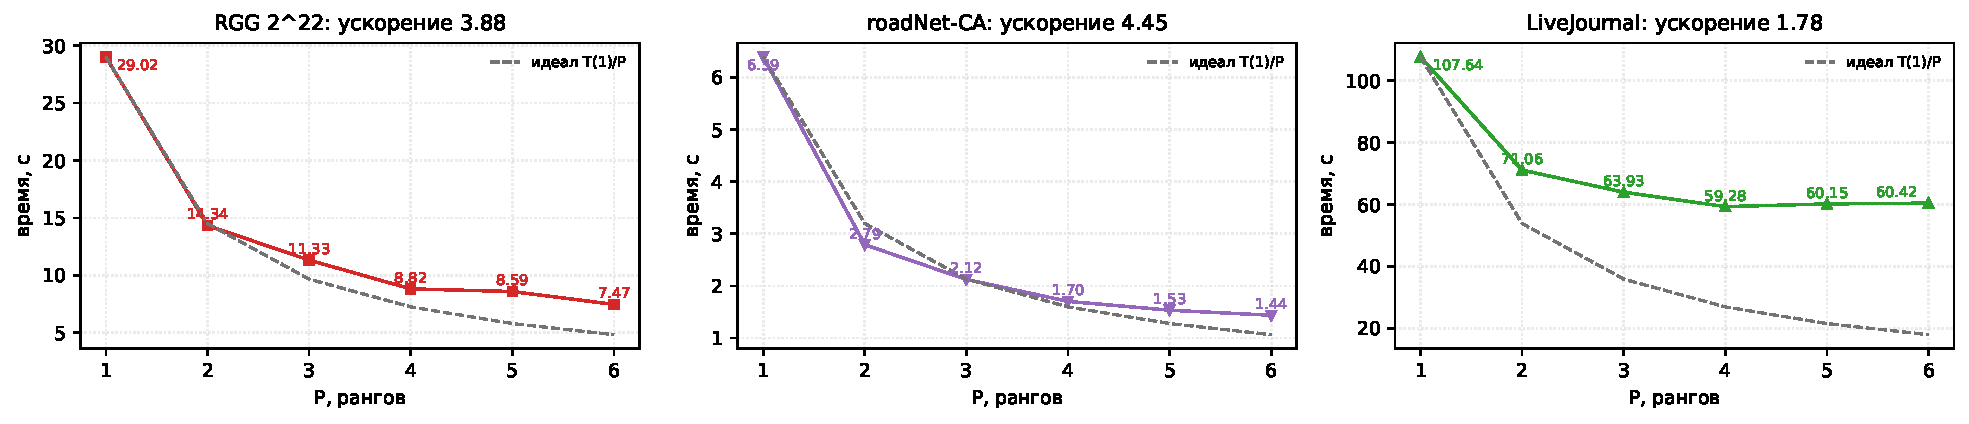
\includegraphics[width=\textwidth,height=.55\textheight,keepaspectratio]{figures/time_pagerank_graphs.pdf}
    \figcap{PageRank: время при $P = 1\ldots6$ рангах, своя панель на каждый граф;
    пунктир~--- идеал $T(1)/P$}

    \begin{itemize}
        \item roadNet-CA: $6.39 \to 1.44$~с, ускорение 4.45~--- лучший результат среди обходов
        \item На однородном графе (дороги Калифорнии) время падает почти линейно
        \item RGG: $29.02 \to 7.47$~с, ускорение 3.88
        \item LiveJournal: $107.64 \to 60.42$~с, ускорение 1.78~--- почти не масштабируется (хабы)
    \end{itemize}
\end{frame}

\begin{frame}[shrink]
    \frametitle{PageRank: время по фазам при разном $P$}
    \centering
    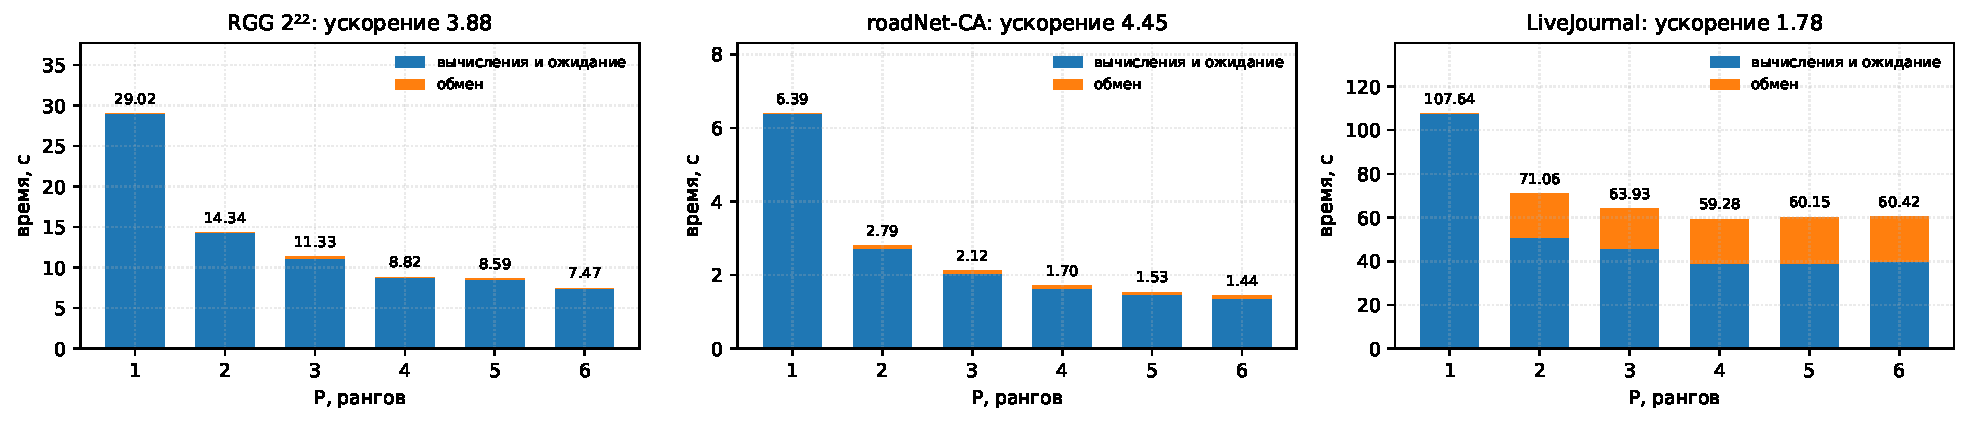
\includegraphics[width=\textwidth,height=.55\textheight,keepaspectratio]{figures/phases_pagerank.pdf}
    \figcap{PageRank: фазы при $P = 1\ldots6$ рангах, медиана 15 прогонов; обмен~---
    \texttt{Gluon Sync\_PageRank\_*}, вычисления и ожидание~--- остаток \texttt{Timer\_N};
    над столбцом~--- время ранга}

    \begin{itemize}
        \item RGG: обмен $\le 2\%$, почти всё время~--- вычисления и ожидание, $S(6) = 3.88$
        \item roadNet-CA: обмен 3--6\%, $S(6) = 4.45$~--- лучший результат среди обходов
        \item LiveJournal: 29--35\%, $S(6) = 1.78$~--- обмен и хабы съедают выигрыш
    \end{itemize}
\end{frame}

\begin{frame}[shrink]
    \frametitle{Подсчёт треугольников: время по графам}
    \centering
    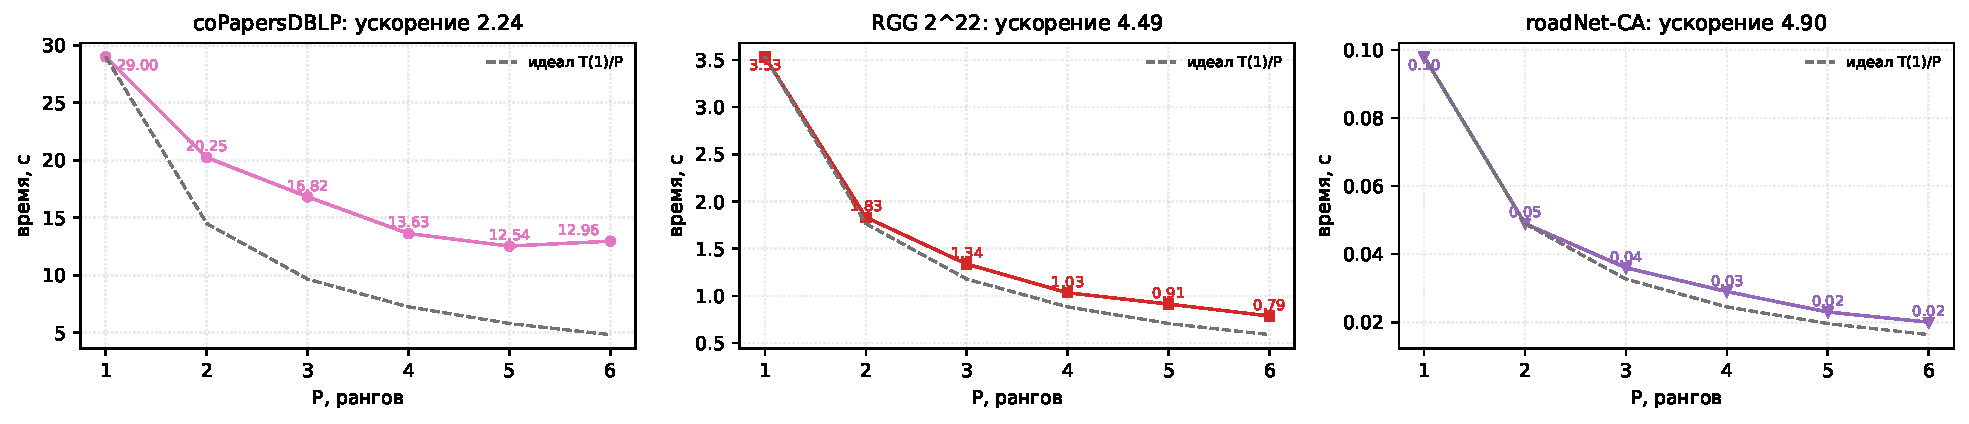
\includegraphics[width=\textwidth,height=.55\textheight,keepaspectratio]{figures/time_tc_graphs.pdf}
    \figcap{TC: время при $P = 1\ldots6$ рангах, своя панель на каждый граф;
    пунктир~--- идеал $T(1)/P$}

    \begin{itemize}
        \item На малых графах масштабируется почти идеально: roadNet-CA $S(6) = 4.90$,
              RGG 4.49~--- один проход по мастерам и одно сложение (Allreduce),
              раундов и обмена нет
        \item coPapersDBLP ($30.5$ млн рёбер): $29.0 \to 13.0$~с, $S(6) = 2.24$
        \item Работа перекошена: времена рангов при $P = 6$~---
              $10.3/13.3/11.6/8.9/6.0/3.1$~с, максимальная степень вершины $6598$
    \end{itemize}
\end{frame}

\begin{frame}
    \frametitle{Результаты}
    \begin{itemize}
        \item Собран стенд: Galois, скрипты запуска и обработки, графики по всем прогонам
        \item Измерены BFS, SSSP, PageRank и TC при $P = 1\ldots6$ на 5 графах
              (по 10--15 прогонов на точку)
        \item Найдено, от чего зависит ускорение:
              \begin{itemize}
                  \item TC делится почти идеально на малых графах ($S(6) = 4.5\ldots4.9$):
                        нет раундов и обмена; на coPapersDBLP с хабами~--- $2.24$
                  \item PageRank делится хорошо на однородных графах (roadNet-CA: 4.45),
                        но плохо на графе с хабами (LiveJournal: 1.78)
                  \item BFS и SSSP ограничены барьером в каждом раунде и обменом зеркалами:
                        $S(6) = 1.3\ldots2.6$
                  \item чем больше средняя степень, тем хуже ускорение:
                        2.5 (belgium\_osm) $\to$ 14.5 (RGG)
                  \item графи с хабами (LiveJournal) почти не ускоряются: 1.26 и 1.31
                  \item промахи кэшей растут с числом рангов ($\times 1.1\ldots5.2$):
                        на LiveJournal копии хабов на всех рангах дают
                        втрое больше промахов, чем при $P = 1$
              \end{itemize}
        \item Ограничения: всё мерили на одной машине (обмен через общую память)
    \end{itemize}
\end{frame}

\end{document}
